
% Options for packages loaded elsewhere
\PassOptionsToPackage{unicode}{hyperref}
\PassOptionsToPackage{hyphens}{url}
%
\documentclass[
]{article}
\usepackage{amsmath,amssymb}
\usepackage{lmodern}
\usepackage{iftex}
\ifPDFTeX
  \usepackage[T1]{fontenc}
  \usepackage[utf8]{inputenc}
  \usepackage{textcomp} % provide euro and other symbols
\else % if luatex or xetex
  \usepackage{unicode-math}
  \defaultfontfeatures{Scale=MatchLowercase}
  \defaultfontfeatures[\rmfamily]{Ligatures=TeX,Scale=1}
\fi
% Use upquote if available, for straight quotes in verbatim environments
\IfFileExists{upquote.sty}{\usepackage{upquote}}{}
\IfFileExists{microtype.sty}{% use microtype if available
  \usepackage[]{microtype}
  \UseMicrotypeSet[protrusion]{basicmath} % disable protrusion for tt fonts
}{}
\makeatletter
\@ifundefined{KOMAClassName}{% if non-KOMA class
  \IfFileExists{parskip.sty}{%
    \usepackage{parskip}
  }{% else
    \setlength{\parindent}{0pt}
    \setlength{\parskip}{6pt plus 2pt minus 1pt}}
}{% if KOMA class
  \KOMAoptions{parskip=half}}
\makeatother
\usepackage{xcolor}
\usepackage[margin=1in]{geometry}
\usepackage{longtable,booktabs,array}
\usepackage{calc} % for calculating minipage widths
% Correct order of tables after \paragraph or \subparagraph
\usepackage{etoolbox}
\makeatletter
\patchcmd\longtable{\par}{\if@noskipsec\mbox{}\fi\par}{}{}
\makeatother
% Allow footnotes in longtable head/foot
\IfFileExists{footnotehyper.sty}{\usepackage{footnotehyper}}{\usepackage{footnote}}
\makesavenoteenv{longtable}
\usepackage{graphicx}
\makeatletter
\def\maxwidth{\ifdim\Gin@nat@width>\linewidth\linewidth\else\Gin@nat@width\fi}
\def\maxheight{\ifdim\Gin@nat@height>\textheight\textheight\else\Gin@nat@height\fi}
\makeatother
% Scale images if necessary, so that they will not overflow the page
% margins by default, and it is still possible to overwrite the defaults
% using explicit options in \includegraphics[width, height, ...]{}
\setkeys{Gin}{width=\maxwidth,height=\maxheight,keepaspectratio}
% Set default figure placement to htbp
\makeatletter
\def\fps@figure{htbp}
\makeatother
\setlength{\emergencystretch}{3em} % prevent overfull lines
\providecommand{\tightlist}{%
  \setlength{\itemsep}{0pt}\setlength{\parskip}{0pt}}
\setcounter{secnumdepth}{-\maxdimen} % remove section numbering
\ifLuaTeX
  \usepackage{selnolig}  % disable illegal ligatures
\fi
\IfFileExists{bookmark.sty}{\usepackage{bookmark}}{\usepackage{hyperref}}
\IfFileExists{xurl.sty}{\usepackage{xurl}}{} % add URL line breaks if available
\urlstyle{same} % disable monospaced font for URLs
\hypersetup{
  pdftitle={Implementation of Sublinear Clustering Algorithm },
  pdfauthor={James Camacho and Joseph Camacho},}

\title{Implementation of Sublinear Clustering Algorithm}
\author{James Camacho and Joseph Camacho}
\date{December 14, 2022}

\begin{document}
\maketitle

\hypertarget{implementation-of-sublinear-clustering-algorithm-rough-draft}{%
  \section{Implementation of Sublinear Clustering Algorithm (Rough
    Draft)}\label{implementation-of-sublinear-clustering-algorithm-rough-draft}}

\hypertarget{by-james-camacho-and-joseph-camacho}{%
  \subsection{By James Camacho and Joseph
    Camacho}\label{by-james-camacho-and-joseph-camacho}}

\hypertarget{introduction}{%
  \subsubsection{Introduction}\label{introduction}}

A (+/-)-graph contains plus-edges and minus-edges, corresponding to positive or negative correlation between two vertices. For example, in a graph of a thesaurus there would be plus-edges between synonyms and minus-edges between antonyms. The clustering problem involves assigning labels to each vertex, trying to assign more highly correlated vertices with the same label. More precisely, a cost function is introduced, with one unit of cost for every pair of correlated vertices assigned different labels and anticorrelated vertices with the same label. In very large, very dense graphs, simply reading every edge can take a very long time, $O(n^2)$ in the number of vertices. We cannot do better than an $\Omega(n)$ algorithm, as every vertex must be assigned a label. This clustering problem is NP, but polynomial approximation schemes are known to exist. In this paper we implement one such approximation scheme by \href{https://doi.org/10.48550/arxiv.2109.14528}{Assadi and Wang} that runs in $\tilde{O}(n)$ time. The running time is $O(n\log^2 n\varepsilon^{-2})$ for some input $\varepsilon$, and it yields an $O(\varepsilon^{-2})$-factor approximation (in terms of cost).

Unfortunately, their theoretical bounds only hold when $\varepsilon < \frac{1}{360}$, which means the algorithm could be off by a factor of $10^5$, not a very practical result. We explore empirically what happens for larger $\varepsilon$, and find more efficient and accurate clustering for $\varepsilon > \frac14$.

\hypertarget{overview}{%
  \subsubsection{Overview}\label{overview}}

We implement Algorithm 1 in
\href{https://doi.org/10.48550/arxiv.2109.14528}{"Sublinear Time and
  Space Algorithms for Correlation Clustering via Sparse-Dense
  Decompositions"} by Sepehr Assadi and Chen Wang. This algorithm implements
correlation clustering, the goal of which is to cluster nodes in a (+/-)-labeled
graph such that the number of +'s between elements of different clusters and
-'s between elements of the same cluster is minimzed. For example, a graph of
all English words could have pluses between synonyms and minuses between
antonyms, and the goal might be to form clusters of semantically related words.
In other datasets, such as document clustering, these graphs can be
incredibly large and dense, leading to a superlinear number of edges
compared to the vertices. On such graphs, even a single pass through the edges can be
infeasible. Assadi and Wang's paper presents an approximation scheme
that uses only {\(\tilde{O}(n)\)} vertices and {\(\tilde{O}(n)\)} edges
(where $\tilde{O}(\cdot)$ is $O(\cdot)$ ignoring logarithmic factors),
which is often sublinear in the size of the input.

It requires access to the plus-labeled edges in an adjacency list, and
works as follows:

\begin{enumerate}
  \tightlist
  \item
        Sample a constant number of edges from each vertex.
  \item
        Choose a random (sublinear) number of vertices and query every edge of
        these vertices.
  \item
        Filter these vertices using the sampled edges from step one to find
        the densest ones.
  \item
        Create candidates for the clusters based on the dense vertices and
        their neighbors.
  \item
        Find approximate clusters from the candidates.
\end{enumerate}

If the constants are chosen right, there should be a high probability
that the candidate clusters in step four form what Assadi and Wang call
a \emph{laminar collection}, a collection of sets for which any two sets
are either disjoint or one is a superset of the other. Then,
step five consists of assigning each vertex to the largest candidate
it's contained in. If it isn't contained
in any candidate clusters, it is assumed to be pretty isolated and
assigned to its own cluster.

We can define a cost for the clustering---each time two vertices are
put in different clusters but have a plus-edge between them, the cost is
increased by one. Similarly if two vertices share a minus-edge but get
put in the same cluster, the cost increases by one. It turns out the
minus-edges are not too relevant, as two vertices with a minus-edge
should only be clustered together if they share a lot of neighbors in
the plus-subgraph, in which case the cost would increase whether or not
they get clustered together. So, by only using the plus-subgraph, it is
possible to determine good clusters with an {\(O(1)\)} approximation to
the optimum.

The accuracy of the algorithm depends on the details. How many edges do
you sample from each vertex? What is the probability you sample all the
edges for a particular vertex? What bounds do you use to filter dense
vertices?

The paper suggests sampling {\(t = O(\varepsilon^{- 2}\log n)\)}
vertices for some small constant {\(\varepsilon\)}. The particular
  {\(\varepsilon\)} is
never explicitly chosen in their paper, but certain theorems of theirs
are proved in the specific case that {\(\varepsilon < 1/360\)}.

In step two, a vertex {\(v\)} is chosen with probability
  {\(O(\log n/\deg(v))\)}. Note that this rewards sparser vertices---in a
complete graph with {\(n\)} vertices you would only expect
  {\(O(\log n)\)} vertices, and thus {\(O(n\log n)\)} edges to be sampled,
while a tree would have nearly every vertex chosen. Overall, steps one
and two only require us to sample
  {\(\tilde{O}(n\varepsilon^{- 2})\)} edges.

The filtering in step three is a little more complicated. First, all
vertices that have many neighbors that are denser than them should be filtered out. This is
according to the formula
  {\[\varepsilon\deg(v) < |\{ u\text{~neighbors~}v:\deg(u) > (1 + \varepsilon)\deg(v)\}|.\]}Then, sparse vertices are filtered out.
Call a neighbor $u$ of $v$ \emph{low} if
  {\[\deg(u) < (1 + 7\varepsilon)\deg(v).\]}A low neighbor {\(u\)} is
\emph{isolated} if
  {\[|\text{sampled\ neighbors}(u) \cap \text{low}(v)| < (1 - 4\varepsilon)t,\]}i.e.
very few of its neighbors are also low neighbors of {\(v\)}. Note that when $\varepsilon > 0.25$, there are no isolated neighbors. When $\varepsilon < 0.25$, we call a vertex \emph{sparse} if at least {\(2\varepsilon\deg(v)\)} of its low neighbors are isolated. Any not-light and not-sparse vertex should be pretty dense.

From here, we use some more magic numbers to build candidate clusters.
For each dense vertex {\(v\)}, we build a candidate set, including a low
neighbor {\(u\)} if
  {\[1 + 22\varepsilon > \frac{\deg(u)}{\deg(v)} > \frac{(1 - 67\varepsilon)t}{|\text{sampled\ neighbors}(u) \cap \text{low}(v)|}.\]}Recall
that there are {\(t\)} sampled neighbors of {\(u\)}, so the right
inequality means that most neighbors of {\(u\)} are also low neighbors
of {\(v\)}. In most of our analysis we have {\(\varepsilon > 1/67\)}, so
this inequality doesn't do much, but it will serve to
increase accuracy as {\(\varepsilon\)} gets very small.

Assadi and Wang claim that, with high probability, these candidate clusters will form a
\emph{laminar set family}, a group of sets where any two elements are either disjoint,
or one is a subset of the other.
If that holds, then we can take the largest disjoint subsets as the clusters.
Any vertices not contained in a subset are assigned as their own cluster.

Our Python implementation can be found on \href{https://github.com/cooljoseph1/Clustering-Algorithm-Implementation}{GitHub}. To measure operations, we create a counter. Every time a function is called, we add the number of operations that call takes within a constant factor. For example, a set `x AND y` operation is known to take $O(\min(x, y))$ time, so we would add $\min(x, y)$ to the counter. To measure error ratios, we find an upper bound for the cost when generating the graph and divide the algorithm's output with this upper bound. This allows larger graphs to be comparable to smaller ones. In the case of the thesaurus, where we do not generate the graph, we simply give the cost. Finally, to determine how far off from laminar the candidate clusters are, we add the sizes of the symmetric differences of every pair of vertices (`len(x XOR y)`), and normalize by dividing by total size and number of vertices.

In this paper we explore more how the choice of {\(\varepsilon\)} and
constant multiplier in {\(t = O(\varepsilon^{- 2}\log n)\)} affect the
operation count and accuracy of the algorithm. We answer questions like,
exactly how close are the candidate clusters to a laminar collection?
How many intersections can we expect? Do we \emph{really} need
  {\(\varepsilon < 1/360\)} in practice, or would larger values like
  {\(\varepsilon = 1/64\)}, {\(\varepsilon = 1/4\)} or
  {\(\varepsilon \approx 1\)} fare equally well? How do sparser or denser
datasets change these results?

\hypertarget{choice-of-varepsilon}{%
  \subsection{\texorpdfstring{Choice of
        {\(\varepsilon\)}}{Choice of \textbackslash varepsilon}}\label{choice-of-varepsilon}}

Assadi and Wang's main result is that their algorithm
results in a constant-approximation of the optimal clustering in
sublinear time (in the number of edges). However, the quality of this constant depends very much
on their choice of {\(\varepsilon\)}, which as we showed above is around $10^5$ when $\varepsilon = 1/360$, the theoretical maximum that guarantees the algorithm works. However, the number of edges we randomly sample per vertex is also proportional to $\varepsilon^{-2}$, so until we have more than $\sim 10^{5}$ vertices and $\sim 10^{10}$ edges, the algorithm runs as slow as reading every single edge, and still isn't guaranteed to do better than a $10^5$ factor approximation. This is terrible!

Luckily, in practice {\(\varepsilon\)} can be raised to much larger
values while maintaining sublinear time in edges, vastly improving the
approximation of the clustering. In order to test this, we use two
datasets. The first is a graph of English words with plus-edges between
synonyms and minus-edges between antonyms. The second is a random graph
with ten thousand vertices, one million edges, and ten clusters; edges
within a cluster are assigned a plus while edges between clusters are
labelled with a minus, however we randomly flip between 10\% and 45\% of
these correlations.

For both datasets running time improved as {\(\varepsilon\)} increased,
as fewer edges needed to be considered. However, the thesaurus dataset
differed from the random dataset with the errors. As {\(\varepsilon\)}
transitioned from less than {\(0.25\)} to more than {\(0.25\)} we saw a
pronounced increase in the number of errors on the real-world data,
while a marked improvement in accurracy for the random dataset. Note
that determining the optimum for the thesaurus dataset is NP-hard, so we
instead give the error count.

\begin{figure}[!htb]
  \center{
    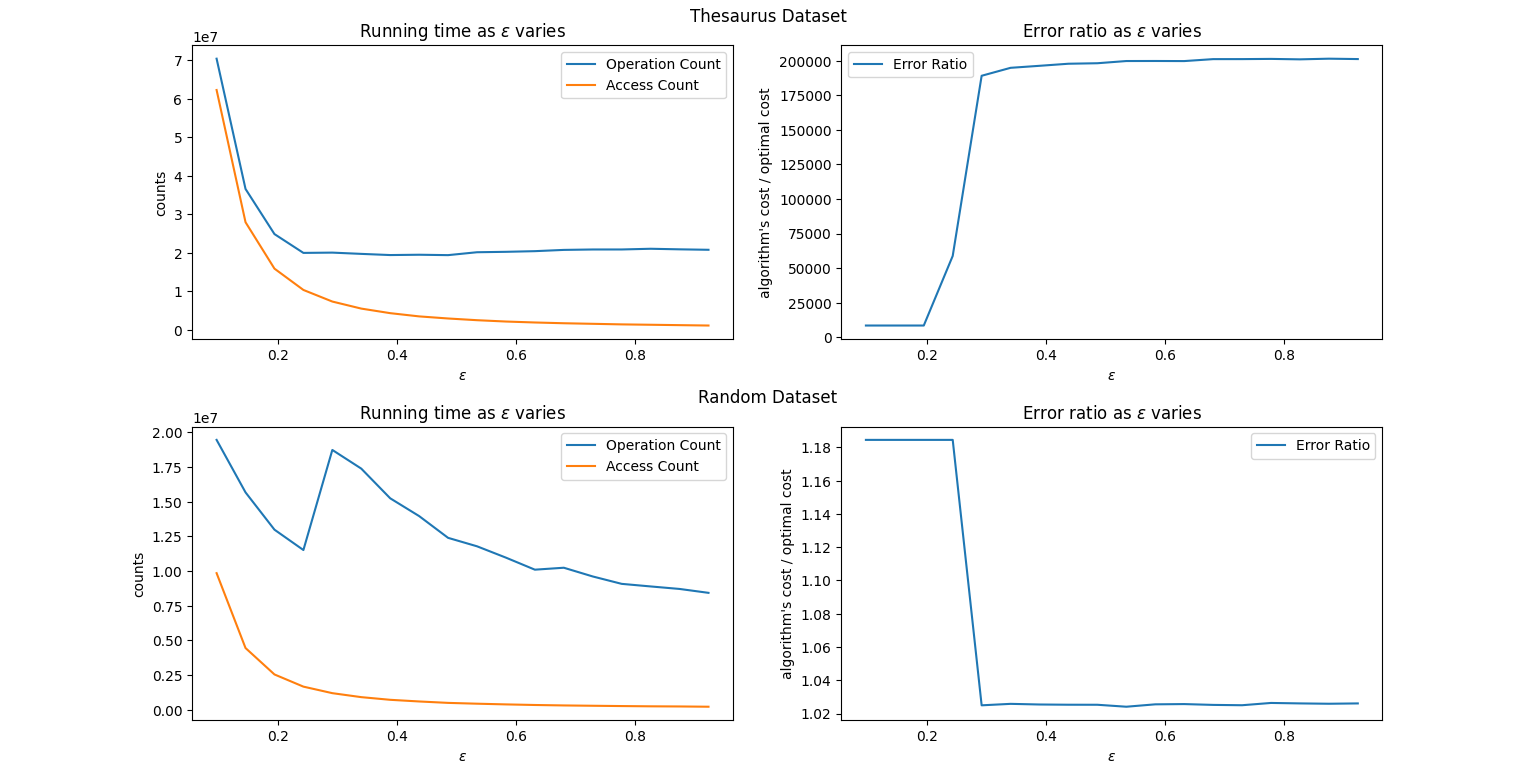
\includegraphics[width=\textwidth]{images/opposite_trends.png}
  }
  \caption{\label{fig:opposite-trends}
    When run on the graph built from a thesaurus (top), the error dramatically increases
    as $\varepsilon$ transitions from less than $0.25$ to more than $0.25$. The exact
    opposite trend is observed on a dataset built from random clusters (bottom).}
\end{figure}
This difference likely arises as there are only \textasciitilde8,000
antonyms compared to \textasciitilde200,000 synonyms in the thesaurus.
Putting all words into one cluster is guaranteed to have very few
errors, while separating into multiple clusters risks synonyms being in
different clusters.

For the random dataset, we see this rapid improvement at
  {\(\varepsilon = 0.25\)} even as we change the fraction of edge
correlations that are flipped, how many clusters there are, or the size
of the graph. For example, the below graphs show the algorithm run with
  {\(\varepsilon = 0.2\)} and {\(\varepsilon = 0.3\)}, and a varying
number of edges, 10\% of which are flipped. Observe that even the least
competitive result when $\varepsilon = 0.3$ is still better than the most
competitive result when $\varepsilon = 0.2$.

\begin{figure}[!htb]
  \begin{tabular}{cc}
    {\(\varepsilon  = 0.2\)} & {\(\varepsilon = 0.3\)}                                           \\
    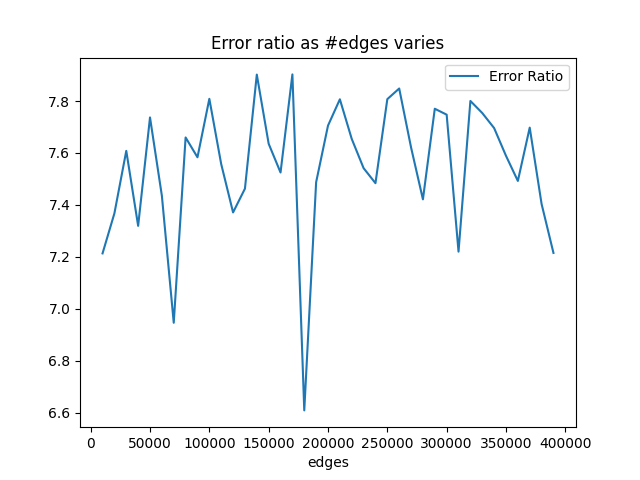
\includegraphics[width=0.5\textwidth]{images/error_ratio_as_edges_varies_eps_equals_0.2.png}
                             &
    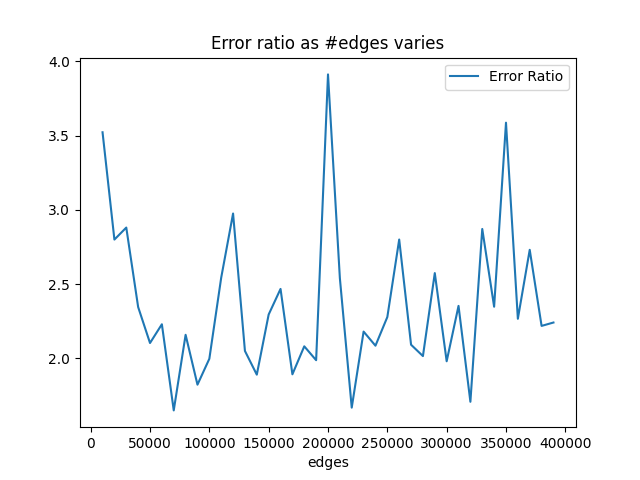
\includegraphics[width=0.5\textwidth]{images/error_ratio_as_edges_varies_eps_equals_0.3.png} \\
  \end{tabular}
  \caption{\label{fig:error-ratio-as-edges-varies}
    For both $\varepsilon = 0.2$ (left) and $\varepsilon = 0.3$ (right), the
    algorithm remains about the same competitive as the number of edges
    increases. However, larger $\varepsilon$ does consistently yield
    a better competitive ratio.}
\end{figure}

Finally, we note that choosing an extremely small $\varepsilon$ gives no improvement
on both the randomly constructed graph and the graph based on the thesaurus. This could be
because such effects are impossible to observe except in very large graphs, since the number
of edges sampled per node is proportional to $\varepsilon^2$. Nevertheless, we think it's
plausible that even in large graphs the optimal choice of $\varepsilon$ is around $0.25$.
Whether $\varepsilon$ should be above or below $0.25$, though, appears to depend on the
structure of the graph.

\begin{figure}[!htb]
  \begin{tabular}{cc}
    {\(\varepsilon  = 0.2\)} & {\(\varepsilon = 0.3\)}                                 \\
    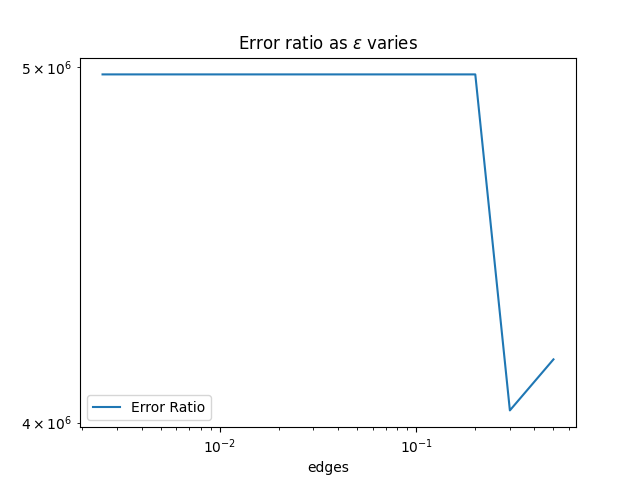
\includegraphics[width=0.5\textwidth]{images/error_ratio_as_eps_varies_loglog_thesaurus.png}
                             &
    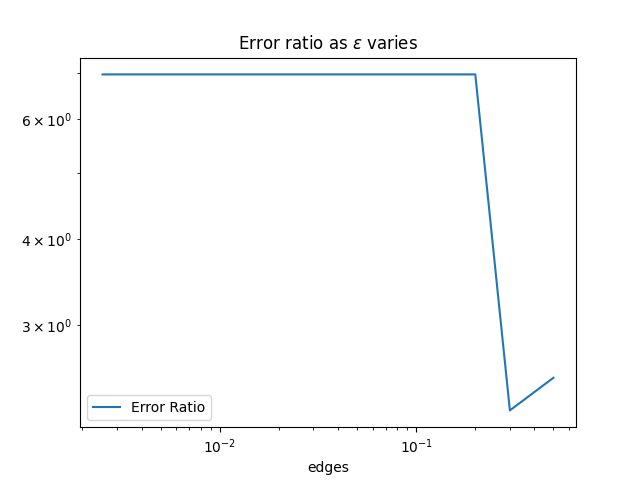
\includegraphics[width=0.5\textwidth]{images/error_ratio_as_eps_varies_loglog.png} \\
  \end{tabular}
  \caption{\label{fig:error-ratio-small-eps}
    In both the thesaurus graph (left) and random graph (right), the error
    ratio fails to improve as $\varepsilon$ is decreased, even when it passes
    criticaldatasets, the error ratio is significantly better for large $\varepsilon$
    For both $\varepsilon = 0.2$ (left) and $\varepsilon = 0.3$ (right), the
    algorithm remains about the same competitive as the number of edges
    increases. However, larger $\varepsilon$ does consistently yield
    a better competitive ratio.}
\end{figure}

\hypertarget{word-vector-dataset}{%
  \subsection{Word Vector Dataset}\label{word-vector-dataset}}


To get a denser model based on real-world data, we create a new dataset
using word vectors. It is well known their dot products are a measure of
correlation, with very positive dot products being highly correlated
while negative dot products are anticorrelated, so we assign plus-edges
to the top percentiles of these dot products, and minus-edges to the
bottom. Changing this fraction allows for sparser or denser graphs.

For all levels of sparsity, we see an error trend similar to that of the
random graphs. Both have optimal clustering when $\varepsilon$ is slightly larger
than $0.25$.
\begin{figure}[!htb]
  \centering{
    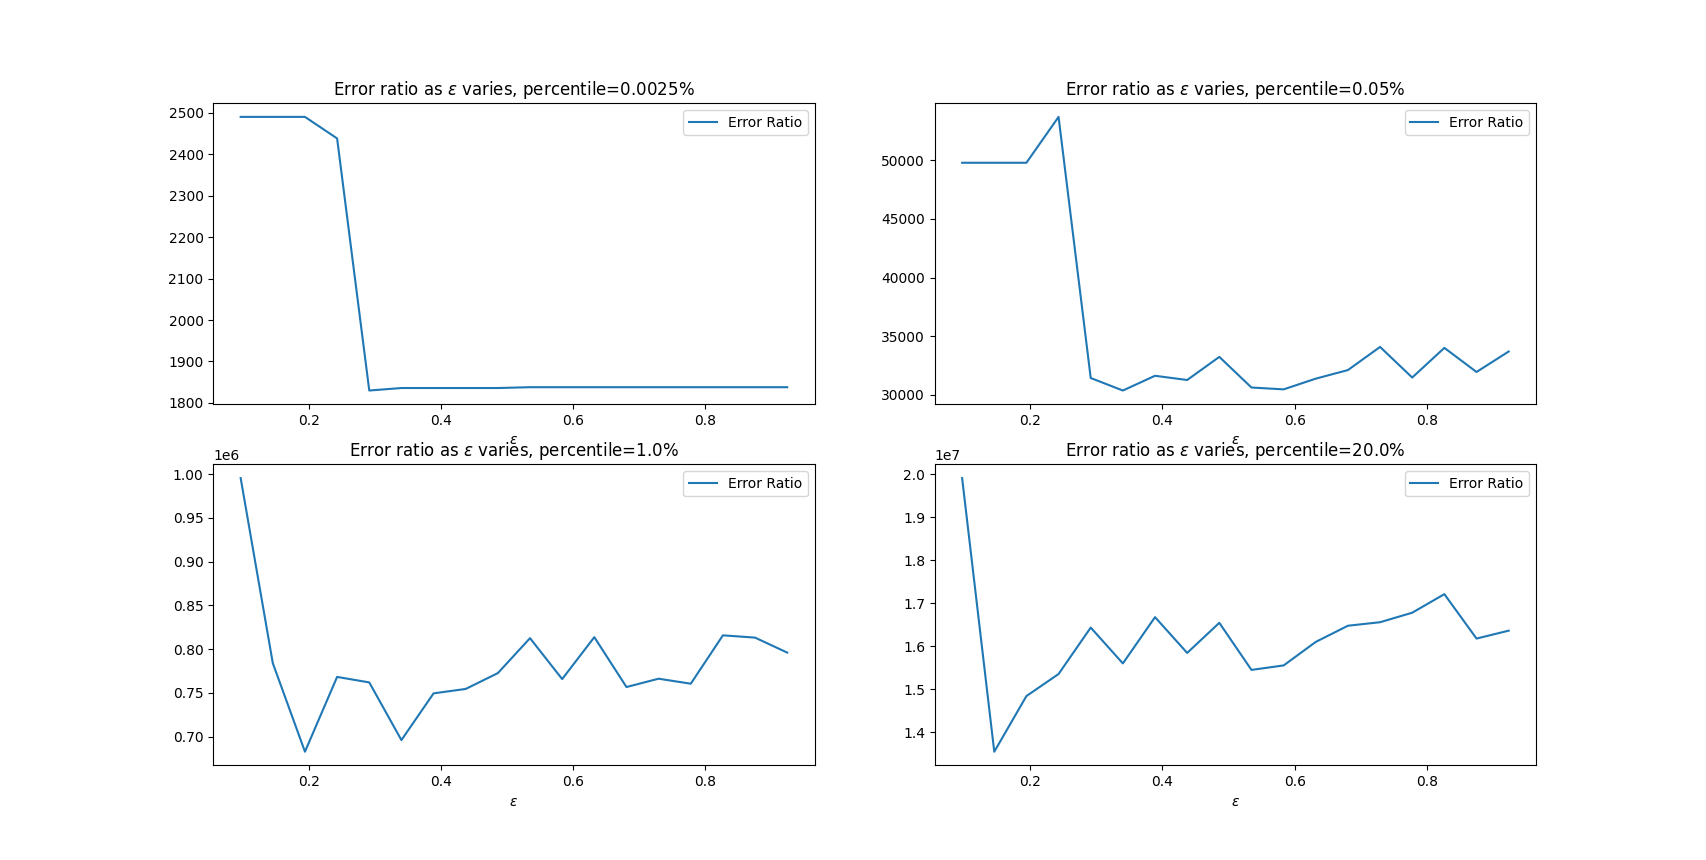
\includegraphics[width=\textwidth]{images/percentile_change.png}
  }
  \caption{\label{fig:percentile-change}
    For a wide range of percentiles, the error trend is similar to that of the
    randomly constructed graphs.}
\end{figure}

Likewise, the running time improves as {\(\varepsilon\)} increases.\\
\begin{figure}[!htb]
  \centering{
    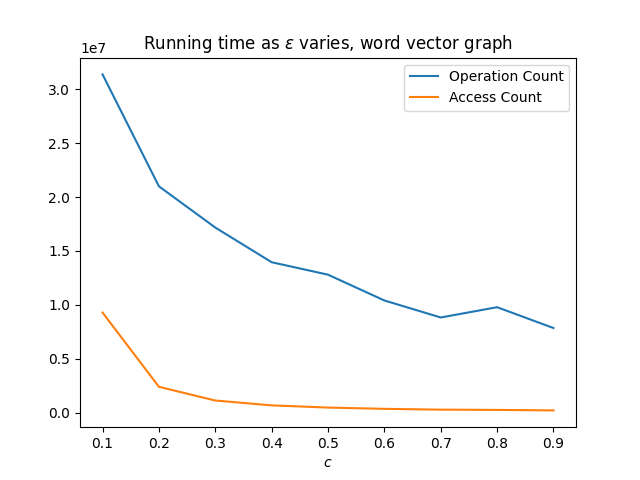
\includegraphics[width=0.5\textwidth]{images/running_time_as_eps_varies_word_vector.png}
  }
  \caption{\label{fig:running-time-word-vector}
    As $\varepsilon$ increases, the running time decreases.}
\end{figure}

This suggests several things, most notably that filtering by isolated
neighbors is actually detrimental to the performance of the algorithm!
Although it's theoretically necessary to do this
filtering to gurantee an {\(O(1)\)} approximation (as the thesaurus
dataset somewhat shows), in practice it's not only
faster to not do so, but also more accurate.

In conclusion, dense graphs from real world data often look similar to the random dataset
we built, and for these types of data, setting {\(\varepsilon\)} to be
slightly more than {\(0.25\)} is a good choice.

\hypertarget{choice-of-c}{%
  \subsection{\texorpdfstring{Choice of
        {\(c\)}}{Choice of c}}\label{choice-of-c}}

In their paper, Assadi and Wang state that "there is an absolute
constant {\(c > 0\)}" for which their algorithm works, but they never
specify exactly what {\(c\)} has to be. In fact, they only imply what
restrictions {\(c\)} might have by constraints on other variables. These
constraints imply that {\(c\)} to be on the order of at least
  {\(\varepsilon^{2}\)}. Since {\(\varepsilon^{2}\)} is rather small, this
means that {\(c\)} can be just about anything.

Nevertheless, setting {\(c = \varepsilon^{2}\)} is hardly useful. While
lowering {\(c\)} speeds up the algorithm by requiring fewer graph
accesses, it also lowers its performance because the algorithm has less
information to make use of. In this section, we explore the tradeoffs of
what {\(c\)} should be, and demonstrate that {\(c \approx 2\)} yields
good results with competitive results.

In the previous section, we showed that a good choice of
  {\(\varepsilon\)} is not much more than {\(0.25\)}. For this section, we
set {\(\varepsilon = 0.3\)}. We find a steep decline in error until a steady increase after $c > 2$.

\begin{figure}[!htb]
  \begin{tabular}{cc}
    Word Vector & Random                                                      \\
    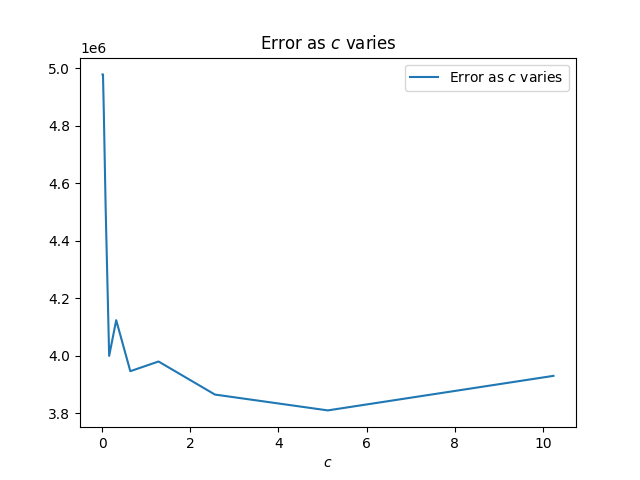
\includegraphics[width=0.5\textwidth]{images/error_ratio_as_c_varies_word_vector.png}
                &
    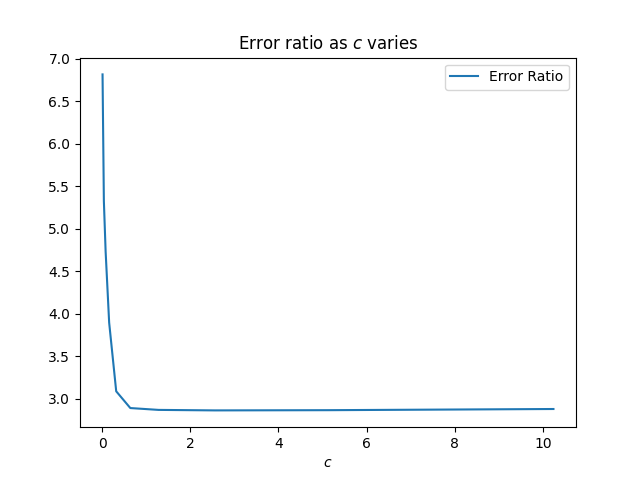
\includegraphics[width=0.5\textwidth]{images/error_ratio_as_c_varies.png} \\
  \end{tabular}
  \caption{\label{fig:error-ratio-c-varies}
    In both the word vector graph (left) and random graph (right), the error
    ratio has a sharp downturn followed by a very slow increase.}
\end{figure}

In both cases, the running time also scales linearly with {\(c\)}. A good trade off, then, between runtime and error ratio appears to be
setting {\(c \approx 2\)}.
\begin{figure}[!htb]
  \centering{
    \begin{tabular}{cc}
      Word Vector & Random                                                       \\
      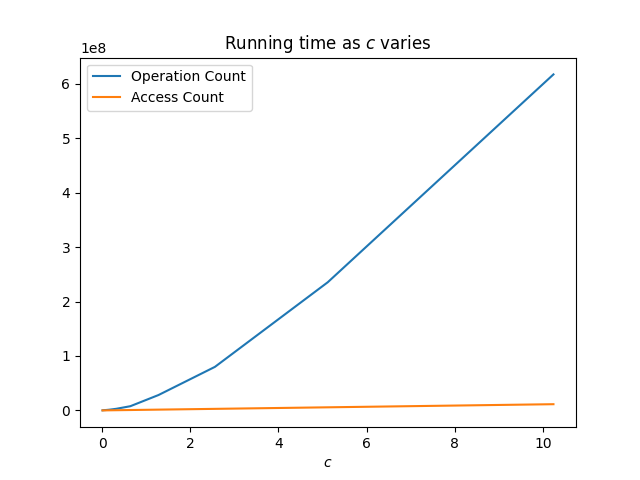
\includegraphics[width=0.5\textwidth]{images/running_time_as_c_varies_word_vector.png}
                  &
      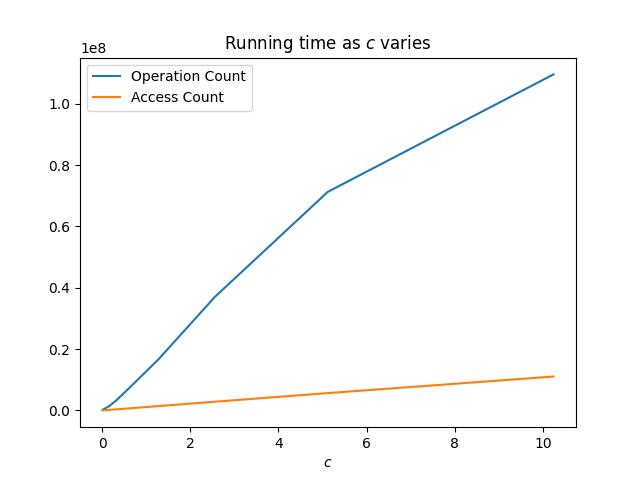
\includegraphics[width=0.5\textwidth]{images/running_time_as_c_varies.png} \\
    \end{tabular}
  }
  \caption{\label{fig:running-time-c-varies}
    As $c$ varies, the running time increases linearly.}
\end{figure}

\hypertarget{sublinear-time}{%
  \subsection{Sublinear Time}\label{sublinear-time}}

In their paper, Assadi and Wang mathematically proved that their algorithm
runs in sublinear time in the number of edges for small enough $\varepsilon$.
Specifically, they showed it ran in $O(|V| \log^2 |V|)$ time, where $|V|$
is the number of vertices of the graph. In this section, we explore whether
this same relation holds for much larger $\varepsilon$---$\varepsilon$ around
$0.25$---and a fixed $c = 2$. (Unfortunately, we don't have the compute available
to empirically show their bound holds true for $\varepsilon < 1 / 360$.)

To do this, we observe the runtimes of the algorithm on two graphs with 10,000
vertices and a varying number of edges---one random graph and one graph made
from word vectors. We see a what might be a concave trend, although it's difficult to
tell whether it truly is sublinear at this scale.

\begin{figure}[!htb]
  \centering{
    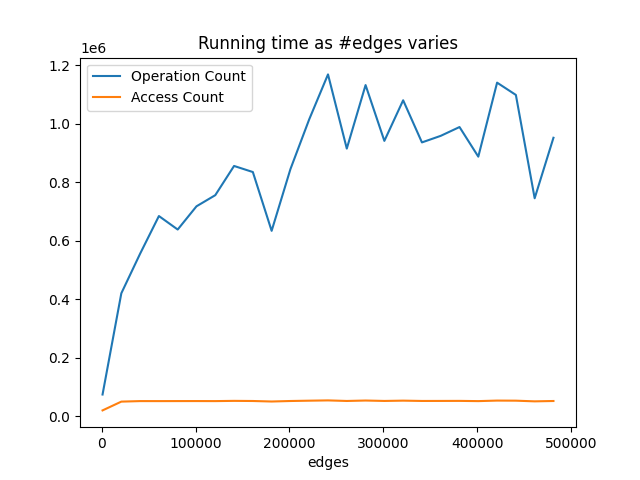
\includegraphics[width=0.45\textwidth]{images/running_time_as_edges_varies.png}
    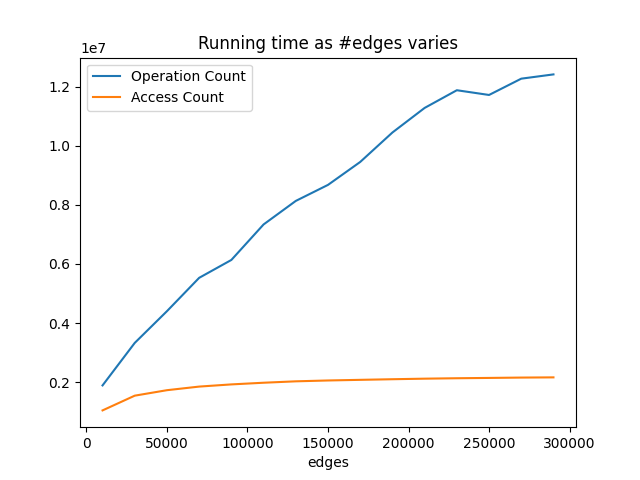
\includegraphics[width=0.45\textwidth]{images/running_time_as_edges_varies_word_vector.png}
  }
  \caption{\label{fig:running-time-c-varies}
    As the number of edges vary in the random graph (left) and word vector graph (right),
    the running time grows, possibly sub-linearly.}
\end{figure}

\hypertarget{laminar-candidate-clusters}{%
  \subsection{Laminar Candidate
    Clusters}\label{laminar-candidate-clusters}}

Assadi and Wang make the claim that the candidate clusters have a high
probability of forming a laminar set family. Every pair of candidates
should either be disjoint, or one is a subset of the other. Suppose two
candidates do not satisfy this laminar property. Their symmetric
difference is all elements contained in exactly one subset but not the
other, and so the sum of the symmetric differences is a measure of how
far off from laminar the candidates are. Normalizing by number of
vertices and number of candidate sets gives the graphs in figures \ref{fig:laminar-error-random-graph} and \ref{fig:laminar-error-word-vector-graph}.

\begin{figure}[!htb]
  \begin{tabular}{cc}
    {\(c = 2\)} is fixed, {\(\varepsilon\)} varies. & {\(\varepsilon = 0.3\)} is fixed, {\(c\)} varies. \\
    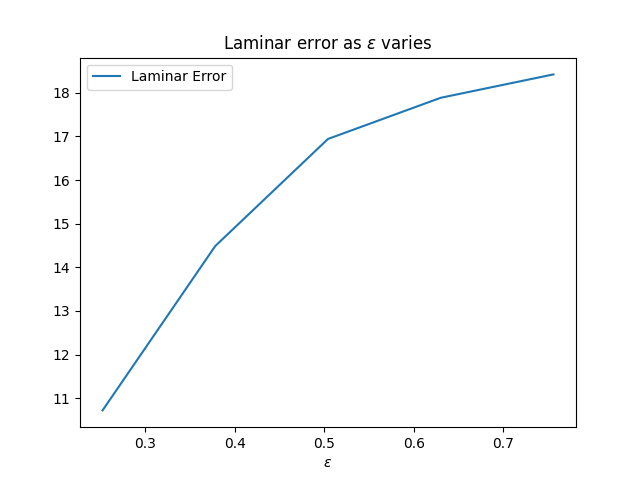
\includegraphics[width=0.5\textwidth]{images/laminar_error_as_epsilon_varies.png}
                                                    &
    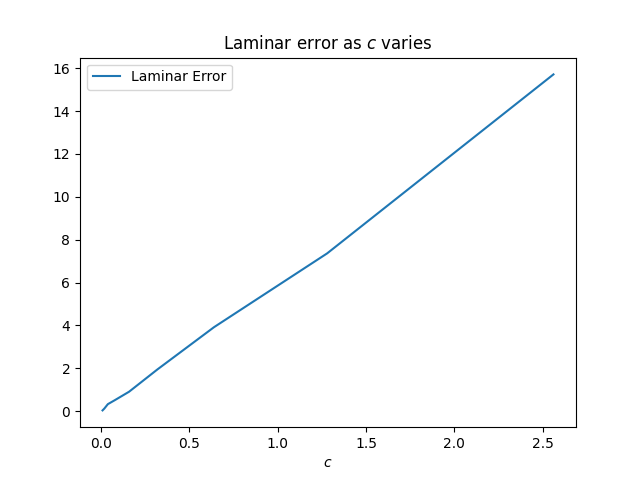
\includegraphics[width=0.5\textwidth]{images/laminar_error_as_c_varies.png}                         \\
  \end{tabular}
  \caption{\label{fig:laminar-error-random-graph}
    As we increase $\varepsilon$ (left) or $c$ (right), the laminar error increases for our random graph with $10^4$ vertices, $10^6$ edges, ten clusters, and $10\%$ edge flip probability.}
\end{figure}

\begin{figure}[!htb]
  \begin{tabular}{cc}
    {\(c = 2\)} is fixed, {\(\varepsilon\)} varies. & {\(\varepsilon = 0.3\)} is fixed, {\(c\)} varies. \\
    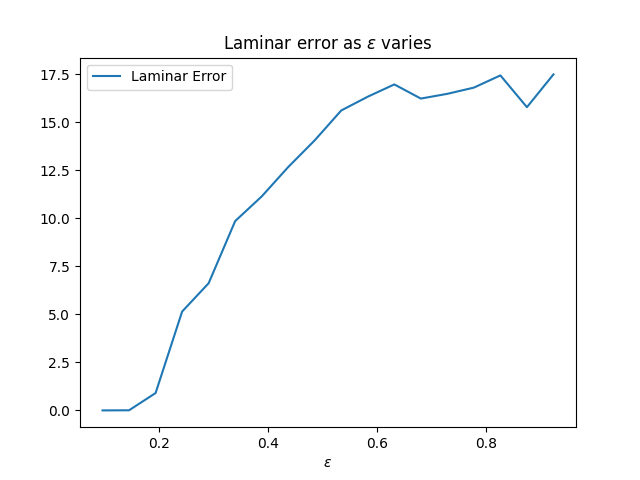
\includegraphics[width=0.5\textwidth]{images/laminar_error_as_epsilon_varies_word_vector.png}
                                                    &
    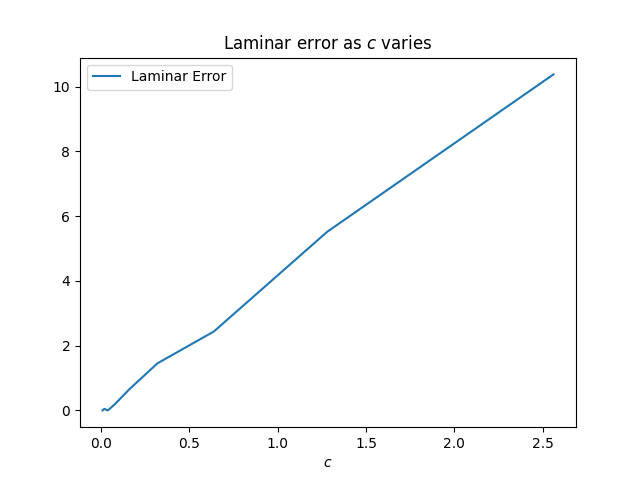
\includegraphics[width=0.5\textwidth]{images/laminar_error_as_c_varies_word_vector.png}             \\
  \end{tabular}
  \caption{\label{fig:laminar-error-word-vector-graph}
    As we increase $\varepsilon$ (left) or $c$ (right), the laminar error increases for our word vector graph with $10^4$ vertices and $5\cdot 10^6$ edges.}
\end{figure}

For both graphs we see an approximately linear increase in laminar error as {\(c\)}
increases, and sublinear increase for {\(\varepsilon\)}. From our
earlier analysis, for graphs of this size we want
  {\(\varepsilon \approx 0.3\)} and {\(c \approx 2\)}, which would give
the average vertex at most ten potential clusters, around {\(1\%\)} of
the total number of clusters, narrowing down potential clusters tremendously. In our implementation we assigned vertices to one of these clusters arbitrarily, but it would be interesting for future work to create a better algorithm for assigning clusters in the final step.

\hypertarget{conclusion}{%
  \subsection{Conclusion}\label{conclusion}}

In this paper, we implemented Sepehr Assadi and Chen
Wang's algorithm for correlation clustering. Although they only proved theoretical results when $\varepsilon < 1/360$, we empirically found a dip in error just above $\varepsilon = 0.25$. This suggests the sparse vertex filtering from step three dramatically reduces the accuracy for a small speedup in running time. When $\varepsilon\approx 0.3$ we found an error ratio of approximately ten times the cost for our graph with 10 million edges, much better than the theoretical $10^5$-factor for $\varepsilon = 1/360$. For this $\varepsilon$, we found that setting $c = 2$ gave a good tradeoff between accuracy and run time. In addition, each vertex had approximately ten different clusters it could belong to. These are incredibly good results, sorting vertices into the top 1\% of all clusters. It would be interesting to see a future algorithm employ a recursive strategy here. Altogether, these results hint that there's a yet-to-be-discovered algorithm with near optimal cost and sublinear running time in the number of edges.

\hypertarget{references}{%
  \subsection{References}\label{references}}

\href{https://doi.org/10.48550/arxiv.2109.14528}{"Sublinear Time and
  Space Algorithms for Correlation Clustering via Sparse-Dense
  Decompositions"}

\end{document}
